

Los valores medidos de corriente se convirtieron a amperes y los voltajes se mantuvieron en volts. Primero se graficó $I_a$ como función de $V_a$ para observar la curva característica del diodo. Después se construyó la variable $V_a^{3/2}$ y se realizó un ajuste lineal de $I_a$ contra $V_a^{3/2}$ en el intervalo donde los datos presentaron el comportamiento esperado por la ley de Child--Langmuir.

El ajuste se hizo usando la forma

\begin{equation}
I_a = C V_a^{3/2}
\end{equation}

donde $C$ es la pendiente experimental. Con esta pendiente y con los parámetros geométricos del bulbo 1V2 reportados en la Tabla \ref{tab:parametros_1v2}, se calculó la relación carga-masa del electrón mediante

\begin{equation}
\frac{e}{m_e}
=
\frac{1}{2}
\left(
\frac{9r_a\beta^2 C}{8\pi\varepsilon_0 L}
\right)^2
\end{equation}

Como verificación adicional del régimen de Child--Langmuir, se puede ajustar la relación de potencia

\begin{equation}
I_a = A V_a^p
\end{equation}

mediante la forma linealizada

\begin{equation}
\ln I_a = p\ln V_a + \ln A
\end{equation}

En el régimen limitado por carga espacial, el exponente obtenido debe ser cercano a $p=3/2$.

\begin{center}
    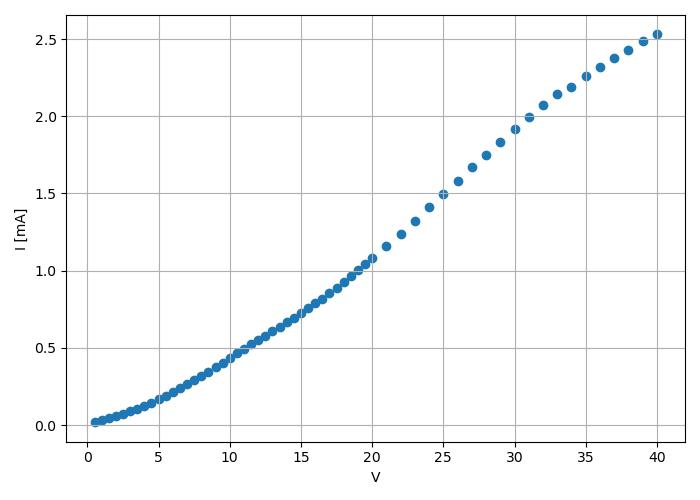
\includegraphics[width=0.92\columnwidth]{figuras/bulbo_datos.jpg}
    \captionof{figure}{Corriente sobre el ánodo al variar su voltaje desde $0-20V$ y $20-40$ en pasos de $0.5V$ y en pasos de $1V$, respectivamente.}
    \label{bulbolimpio}
\end{center}

\begin{center}
    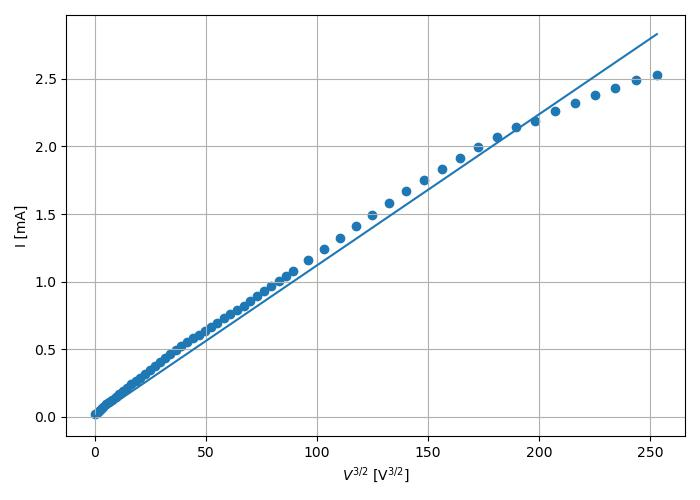
\includegraphics[width=0.92\columnwidth]{figuras/bulbo_ajuste.jpg}
    \captionof{figure}{Ajuste lineal en el origen de los datos de la Figura \ref{bulbolimpio}.}
    \label{bulboajuste}
\end{center}


Para el ajuste en el origen de la forma $I=mx$ donde $I$ sera la corriente, $x = V^{3/2}$ se obtiene 

\begin{table}[h]
\centering
\caption{Parámetros obtenidos del ajuste lineal de \( I\) contra \(V^{3/2}\).}
\begin{tabular}{cc}
\hline
Magnitud & Valor \\
\hline
\(m\) & \((1.11 \pm 0.01)\times10^{-5}\,\mathrm{A/V^{3/2}}\) \\
\(R^2\) & \(0.995\) \\
\(e/m_e\) & \((1.719 \pm 0.032)\times10^{11}\,\mathrm{C/kg}\) \\
\(E\%\) & \(-2.23\%\) \\
\hline
\end{tabular}
\end{table}

\begin{center}
    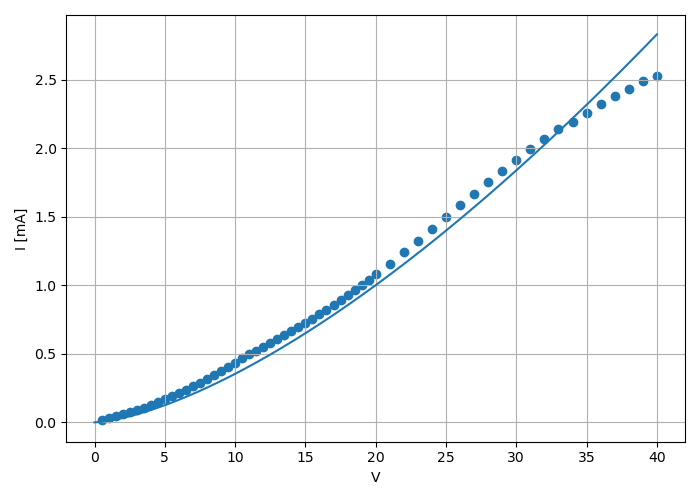
\includegraphics[width=0.92\columnwidth]{figuras/bulbo_sobre_ajuste.png}
    \captionof{figure}{Ajuste en potencia de los datos de la Figura \ref{bulbolimpio}.}
    \label{bulboajuste_limpio}
\end{center}


Para el ajuste linealizado $\ln I = p \ln V + \ln m$ se obtiene 

\begin{table}[h]
\centering
\caption{Parámetros obtenidos del ajuste lineal de \( \ln I\) contra \(V\).}
\begin{tabular}{cc}
\hline
Magnitud & Valor \\
\hline
\(p\) & \(1.243 \pm 0.013\) \\
$m$ & \((2.57 \pm  0.09)\times 10^{-5}\,A/V^p\)\\
\(R^2\) & \(0.993\) \\
\(E\%\) & \(-17.1\%\) \\
\hline
\end{tabular}
\end{table}

\begin{center}
    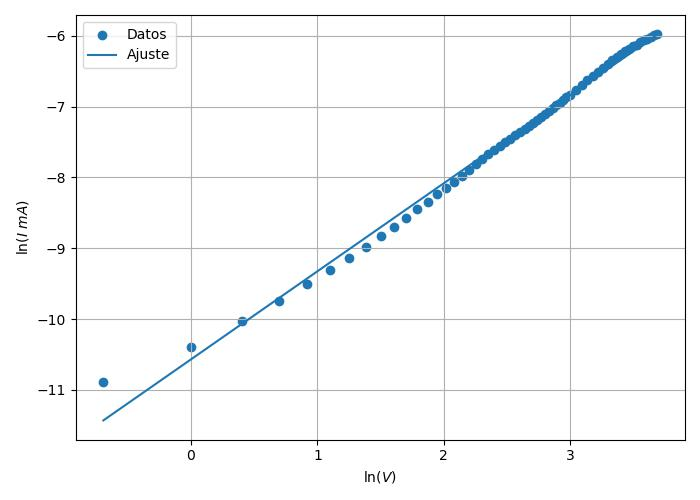
\includegraphics[width=0.92\columnwidth]{figuras/tresmedios.jpg}
    \captionof{figure}{Ajuste linealizado de los datos de la Figura \ref{bulbolimpio}.}
    \label{bulbolineal}
\end{center}
